\documentclass[
  11pt,
  letterpaper,
   addpoints,
  answers
  ]{exam}

% Carga el preámbulo localizado en la carpeta superior
\NeedsTeXFormat{LaTeX2e}[2023/04/30]

% Provide the name of your page, the date it was last updated, and a comment about what it's used for
\ProvidesPackage{../exercise-preamble}[2023/04/30 Prof. Cassanelli custom LaTeX style]

% \usepackage{printlen}
% \uselengthunit{in}\printlength{\textwidth}

% PACKAGES
\usepackage[dvipsnames]{xcolor}

\usepackage{graphicx}
\graphicspath{{../figures}}
\usepackage{amsmath,amsthm,amssymb,mathtools,mathrsfs}
\usepackage{commath}
\usepackage{upgreek}
\usepackage{cancel}
\usepackage{enumerate}
\usepackage[font=small]{caption}
\usepackage[normalem]{ulem}
\usepackage{steinmetz}

\usepackage[left=1.5cm, right=1.5cm, top=1cm]{geometry}

% REFERENCES AND OTHERS
\usepackage{../aas_macros}
\usepackage{natbib}
\bibpunct{(}{)}{;}{a}{}{,}

\usepackage{tikz}
\usepackage{tikz-3dplot}
\usepackage{circuitikz}
\usepackage{pgfplots}
\pgfplotsset{compat=1.15}
\usepgfplotslibrary{smithchart}
\usetikzlibrary{
  decorations.pathmorphing,
  decorations.markings,
  calc,
  patterns,
  decorations,
  angles,
  quotes,
  ext.topaths.arcthrough,
  shapes
  }

\usepackage{siunitx}
\sisetup{
    range-phrase=\text{--},
    range-units=single,
    separate-uncertainty=true,
    print-unity-mantissa=false
    }
\DeclareSIUnit{\gauss}{G}
\DeclareSIUnit{\jansky}{Jy}

\newcommand{\iu}{\mathrm{i}\mkern1mu}
\newcommand{\ju}{\mathrm{j}\mkern1mu}
\newcommand{\euler}{\mathrm{e}}
\newcommand{\exponential}[1]{\mathrm{exp}\left[#1\right]}
\newcommand{\uvec}[1]{\widehat{\mathbf{#1}}}
\newcommand{\uvecs}[1]{\boldsymbol{\widehat{#1}}}
\newcommand{\bvec}[1]{\boldsymbol{\mathcal{#1}}}

\usepackage{hyperref}
\hypersetup{
    % bookmarks=true,
    unicode=true,
    pdftoolbar=true,
    pdfmenubar=true,
    pdffitwindow=false,
    pdfstartview={FitH},
    pdftitle={EL3103},
    pdfauthor={Tomas Cassanelli},
    pdfcreator={Tomas Cassanelli},
    pdfnewwindow=true,
    colorlinks=true,
    linkcolor=Violet,
    citecolor=Violet,
    urlcolor=Violet
    }

% Exam document class
\renewcommand{\figurename}{Figura}
\renewcommand{\tablename}{Cuadro}
\pagestyle{empty}

\usepackage[spanish]{cleveref}

\crefname{question}{\protect{pregunta}}{\protect{preguntas}}
\Crefname{question}{\protect{Pregunta}}{\protect{Preguntas}}
\creflabelformat{question}{#2{#1}#3}

\renewcommand{\solutiontitle}{\noindent\textbf{Solución:}\par\noindent}
\bracketedpoints
\pointname{~puntos}

\endinput

% Paquetes locales
\usepackage{float}
\usepackage{booktabs} % para \toprule, \midrule, \bottomrule
\usepackage{xcolor} % para colores
\usepackage{bm} % para negrita en símbolos matemáticos

% Macros locales
\newcommand{\Rel}{\mathfrak{R}} % símbolo para la reluctancia
\DeclareMathOperator{\Var}{Var} % operador de varianza

\begin{document}

% Configuración del encabezado usando comandos de la clase exam
\pagestyle{headandfoot}
\extraheadheight{0.5in} % Baja el encabezado aumentando el espacio superior
\firstpageheader{\textit{Análisis de Sistemas Dinámicos y Estimación}}{}{EL3204-1}
\runningheader{\textit{Análisis de Sistemas Dinámicos y Estimación}}{}{EL3204}
\firstpagefooter{}{\thepage}{}
\runningfooter{}{\thepage}{}
\headrule % Línea debajo del encabezado

% Numeración de página
\pagenumbering{arabic}

% Portada
\begin{center}
    \vspace*{1cm}
    
    % Logo superior
    \includegraphics[width=0.5\textwidth]{../fcfm_die}
    
    \vspace{2cm}
    
    % Líneas decorativas superiores
    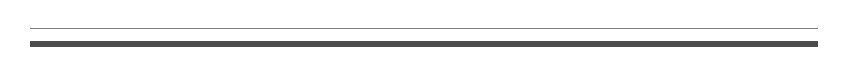
\begin{tikzpicture}
        \draw[line width=2pt, black!70] (0,0) -- (10,0);
        \draw[line width=0.5pt, black!50] (0,0.2) -- (10,0.2);
    \end{tikzpicture}
    
    \vspace{1cm}
    
    % Título principal
    {\fontsize{28}{34}\selectfont\bfseries 
    Análisis de Sistemas\\[0.3cm]
    Dinámicos y Estimación}
    
    \vspace{0.5cm}
    
    {\Large\textbf{EL3204-1}}
    
    \vspace{1cm}
    
    % Líneas decorativas inferiores
    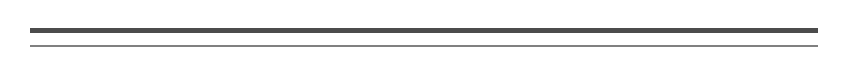
\begin{tikzpicture}
        \draw[line width=0.5pt, black!50] (0,0) -- (10,0);
        \draw[line width=2pt, black!70] (0,0.2) -- (10,0.2);
    \end{tikzpicture}
    
    \vspace{1.5cm}
    
    % Subtítulo
    {\LARGE\itshape Pauta Auxiliar 11 - Estimación}
    
    \vspace{0.5cm}
    {\large Prof Marcos Orchard - Sebastian Espinoza.}\\
    {\large Prof Auxiliar Erik Sáez Aravena.}
    
    % Decoración con símbolo matemático de fondo
    \begin{tikzpicture}[remember picture, overlay]
        \node[opacity=0.5, rotate=0] at ([yshift=-8cm]current page.center) {
            \fontsize{280}{300}\selectfont\color{black!15}$\mathcal{I}(\theta)$
        };
    \end{tikzpicture}
    
    \vfill
    
\end{center}

\newpage
%----------------------------
% =========================================
% Unidad III — Estimación de Parámetros (Resumen)
% =========================================
\section*{Resumen}

Este auxiliar cubre conceptos fundamentales de la teoría de estimación de parámetros, que complementa los temas de detección vistos anteriormente. En problemas de detección, el espacio paramétrico $\Theta$ era discreto y finito, pero ahora trabajamos con un conjunto \textbf{infinito no numerable} de posibles valores para el parámetro que queremos estimar (un continuo).

\subsection*{1. Conceptos Básicos de Estimación}
Algunos conceptos importante a considerar son:
\begin{enumerate}
\item \textbf{Espacio de observación ($\mathbb{X}$):} Espacio donde la variable aleatoria $X \in \mathbb{X}$ toma valores. Para vectores aleatorios, $\mathbb{X}^n$ representa el espacio producto.

  \item  \textbf{Espacio de decisión ($\Theta$):} En estimación, es un conjunto \textbf{infinito no numerable} de valores (a diferencia de detección donde era finito). Ejemplos: $\Theta = \mathbb{R}^+$ para estimar amplitudes, $\Theta = \mathbb{R}$ para estimar medias.

\item \textbf{Familia de distribuciones paramétricas ($J_\theta$):} Conjunto de distribuciones indexadas por $\theta$:
\[
J_\theta = \{P_X(x|\theta) : \theta \in \Theta\}
\]

\item \textbf{Estimador:} Una función $\hat{\theta}(x_1, \ldots, x_n)$ que depende de las observaciones y entrega una estimación del parámetro $\theta$ asociado a la distribución $P_X(x|\theta)$.
\end{enumerate}
\subsection*{2. Propiedades de los Estimadores}
\begin{enumerate}
  \item \textbf{Estimador Insesgado:} Un estimador $\hat{\theta}(x_1, \ldots, x_n)$ es insesgado si:
\[
\mathbb{E}[\hat{\theta}(X_1, \ldots, X_n)] = \theta
\]
Es decir, en promedio el estimador entrega el valor verdadero del parámetro.

\item \textbf{Estimador Asintóticamente Insesgado:} Si el sesgo tiende a cero cuando $n \to \infty$:
\[
\lim_{n\to\infty} \mathbb{E}[\hat{\theta}(X_1, \ldots, X_n)] = \theta
\]

\item \textbf{Estimador Consistente:} Un estimador es consistente si converge en probabilidad al valor verdadero:
\[
\lim_{n\to\infty} P_X(|\hat{\theta}(X_1, \ldots, X_n) - \theta| > \epsilon) = 0 \quad \forall \epsilon > 0
\]

\item \textbf{Observación:} Mediante la desigualdad de Chebyshev, si un estimador es insesgado y su varianza tiende a cero cuando $n \to \infty$, entonces es consistente:
\[
\lim_{n\to\infty} \Var(\hat{\theta}(X_1, \ldots, X_n)) = 0 \implies \text{consistencia}
\]
\end{enumerate}
\subsection*{3. Condiciones de Regularidad}

Las condiciones de regularidad permiten intercambiar el orden de derivación e integración en la función de verosimilitud. Bajo estas condiciones se cumple:
\begin{enumerate}
  \item \textbf{Primera condición:} La esperanza de la derivada de la log-verosimilitud es cero:
\[
\mathbb{E}_{X_1^n}\left[\frac{\partial \ln L(X_1, \ldots, X_n|\theta)}{\partial \theta}\right] = 0
\]

\item \textbf{Segunda condición:} La esperanza de un término específico es cero:
\[
\mathbb{E}_{X_1^n}\left[\frac{1}{L(X_1, \ldots, X_n|\theta)}\frac{\partial^2 L(X_1, \ldots, X_n|\theta)}{\partial \theta^2}\right] = 0
\]

\item \textbf{Identidad de Bartlett:} Relaciona la varianza con su segunda derivada:
\[
\mathbb{E}_{X_1^n}\left[\left(\frac{\partial \ln L}{\partial \theta}\right)^2\right] = -\mathbb{E}_{X_1^n}\left[\frac{\partial^2 \ln L}{\partial \theta^2}\right]
\]

Esta identidad permite calcular la información de Fisher de dos formas equivalentes.
\end{enumerate}
\subsection*{4. Información de Fisher}

La información de Fisher $\mathcal{I}(\theta)$ cuantifica cuánta información sobre el parámetro $\theta$ contienen las observaciones:
\[
\mathcal{I}(\theta) = \mathbb{E}\left[\left(\frac{\partial \ln f(X|\theta)}{\partial \theta}\right)^2\right] = -\mathbb{E}\left[\frac{\partial^2 \ln f(X|\theta)}{\partial \theta^2}\right]
\]

\textbf{Propiedad Aditiva:} Para muestras i.i.d., la información de Fisher es aditiva:
\[
\mathcal{I}_n(\theta) = n \cdot \mathcal{I}_1(\theta)
\]

Esta propiedad refleja que más observaciones independientes proporcionan más información sobre el parámetro.

\subsection*{5. Cota de Cramér-Rao}

La cota de Cramér-Rao establece un límite inferior para la varianza de cualquier estimador insesgado:
\[
\Var(\hat{\theta}) \geq \frac{1}{\mathcal{I}(\theta)}
\]
\begin{enumerate}
  \item \textbf{Estimador Eficiente:} Un estimador insesgado que alcanza la cota de Cramér-Rao se llama \textbf{eficiente} o \textbf{de mínima varianza}

\item \textbf{Interpretación:} La información de Fisher es inversamente proporcional a la mínima varianza posible. Más información $\implies$ menor varianza mínima.
\end{enumerate}
\subsection*{6. Estimador de Máxima Verosimilitud (ML)}

El estimador de máxima verosimilitud se obtiene maximizando la función de verosimilitud:
\[
\hat{\theta}_{ML} = \arg\max_{\theta} L(x_1, \ldots, x_n|\theta) = \arg\max_{\theta} \ln L(x_1, \ldots, x_n|\theta)
\]

\textbf{Propiedades del estimador ML:}
\begin{itemize}
    \item Bajo condiciones de regularidad, es asintóticamente insesgado
    \item Es consistente
    \item Es asintóticamente eficiente (alcanza la cota de Cramér-Rao cuando $n \to \infty$)
    \item Es invariante bajo transformaciones: si $\hat{\theta}_{ML}$ es el ML de $\theta$, entonces $g(\hat{\theta}_{ML})$ es el ML de $g(\theta)$
\end{itemize}

\textbf{Método de solución:} Criterio de la primera derivada:
\[
\frac{\partial \ln L(x_1, \ldots, x_n|\theta)}{\partial \theta}\bigg|_{\theta=\hat{\theta}_{ML}} = 0
\]

Verificar que la segunda derivada es negativa para confirmar que es un máximo.

\subsection*{7. Resumen de Verificaciones para un Estimador}

Para analizar completamente un estimador $\hat{\theta}$, verificar:

\begin{enumerate}
    \item \textbf{Insesgamiento:} Calcular $\mathbb{E}[\hat{\theta}]$ y verificar si es igual a $\theta$
    \item \textbf{Consistencia:} Verificar que $\lim_{n\to\infty} \Var(\hat{\theta}) = 0$ (si es insesgado)
    \item \textbf{Varianza:} Calcular $\Var(\hat{\theta})$ explícitamente
    \item \textbf{Eficiencia:} Calcular $\mathcal{I}(\theta)$ y comparar $\Var(\hat{\theta})$ con $\frac{1}{\mathcal{I}(\theta)}$
\end{enumerate}

%----------------------------
\newpage
\begin{questions}
\question
\label{q:regularidad}
Bajo las condiciones de regularidad de la Definición 3.2 del apunte, verifique si el vector aleatorio $X_1, \ldots, X_n$ es i.i.d. con distribución $P_{X_1^n}(\cdot|\theta)$ entonces
\begin{equation}
\mathbb{E}_{X_1^n}\left(\left(\frac{\partial \ln L(X_1, \ldots, X_n|\theta)}{\partial \theta}\right)^2\right) = -\mathbb{E}_{X_1^n}\left(\frac{\partial^2 \ln L(X_1, \ldots, X_n|\theta)}{\partial \theta^2}\right). \label{eq:regularidad}
\end{equation}

\begin{solution}
Para demostrar esta identidad, utilizaremos las siguientes condiciones de regularidad que permiten intercambiar el orden de derivación e integración:

\textbf{Primera condición de regularidad:} La esperanza de la primera derivada de la log-verosimilitud es cero:
\begin{equation}
\mathbb{E}_{X_1^n}\left[\frac{\partial \ln L(X_1, \ldots, X_n|\theta)}{\partial \theta}\right] = 0
\end{equation}

\textbf{Segunda condición de regularidad:}La esperanza de un término específico es cero:
\begin{equation}
\mathbb{E}_{X_1^n}\left[\frac{1}{L(X_1, \ldots, X_n|\theta)}\frac{\partial^2 L(X_1, \ldots, X_n|\theta)}{\partial \theta^2}\right] = 0
\end{equation}

Partimos de la primera condición de regularidad:
\[
\mathbb{E}_{X_1^n}\left[\frac{\partial \ln L(X_1, \ldots, X_n|\theta)}{\partial \theta}\right] = 0
\]

Y derivamos ambos lados de esta ecuación respecto a $\theta$. Del lado izquierdo, bajo condiciones de regularidad podemos intercambiar la derivada con la esperanza (que es una integral):
\[
\frac{\partial}{\partial \theta}\underbrace{\mathbb{E}_{X_1^n}\left[\frac{\partial \ln L(X_1, \ldots, X_n|\theta)}{\partial \theta}\right]}_{= 0} = \mathbb{E}_{X_1^n}\left[\frac{\partial^2 \ln L(X_1, \ldots, X_n|\theta)}{\partial \theta^2}\right]
\]

Del lado derecho, derivamos la constante $0$:
\[
\frac{\partial}{\partial \theta}(0) = 0
\]

Por lo tanto:
\[
\mathbb{E}_{X_1^n}\left[\frac{\partial^2 \ln L(X_1, \ldots, X_n|\theta)}{\partial \theta^2}\right] = 0
\]

Este resultado nos dice que la esperanza de la segunda derivada de la log-verosimilitud es cero. Ahora necesitamos conectar estos dos resultados. Partimos de la propiedad fundamental del logaritmo aplicada a la función de verosimilitud:
\[
\frac{\partial \ln L(X_1, \ldots, X_n|\theta)}{\partial \theta} = \frac{1}{L(X_1, \ldots, X_n|\theta)}\frac{\partial L(X_1, \ldots, X_n|\theta)}{\partial \theta}
\]

Ahora derivamos ambos lados respecto a $\theta$ para obtener la segunda derivada. Aplicamos la regla del producto en el lado derecho, donde tenemos un producto de dos funciones: $\frac{1}{L(X_1, \ldots, X_n|\theta)}$ y $\frac{\partial L(X_1, \ldots, X_n|\theta)}{\partial \theta}$. Recordemos la regla del producto: si $h(\theta) = f(\theta) \cdot g(\theta)$, entonces $\frac{dh}{d\theta} = \frac{df}{d\theta} \cdot g + f \cdot \frac{dg}{d\theta}$.

Aplicando esto a lo siguiente:
\[
\frac{\partial^2 \ln L(X_1, \ldots, X_n|\theta)}{\partial \theta^2} = \frac{\partial}{\partial \theta}\left[\frac{1}{L(X_1, \ldots, X_n|\theta)}\frac{\partial L(X_1, \ldots, X_n|\theta)}{\partial \theta}\right]
\]

Desarrollamos usando la regla del producto:
\[
= \underbrace{\frac{\partial}{\partial \theta}\left(\frac{1}{L(X_1, \ldots, X_n|\theta)}\right)}_{\text{derivada del primer factor}} \cdot \frac{\partial L(X_1, \ldots, X_n|\theta)}{\partial \theta} + \frac{1}{L(X_1, \ldots, X_n|\theta)} \cdot \underbrace{\frac{\partial^2 L(X_1, \ldots, X_n|\theta)}{\partial \theta^2}}_{\text{derivada del segundo factor}}
\]

Para el primer término, calculamos la derivada de $\frac{1}{L(X_1, \ldots, X_n|\theta)}$ usando la regla de la cadena:
\[
\frac{\partial}{\partial \theta}\left(\frac{1}{L(X_1, \ldots, X_n|\theta)}\right) = -\frac{1}{L(X_1, \ldots, X_n|\theta)^2}\frac{\partial L(X_1, \ldots, X_n|\theta)}{\partial \theta}
\]

Sustituyendo esto en la expresión anterior:
\[
\frac{\partial^2 \ln L(X_1, \ldots, X_n|\theta)}{\partial \theta^2} = -\frac{1}{L(X_1, \ldots, X_n|\theta)^2}\left(\frac{\partial L(X_1, \ldots, X_n|\theta)}{\partial \theta}\right)^2 + \frac{1}{L(X_1, \ldots, X_n|\theta)}\frac{\partial^2 L(X_1, \ldots, X_n|\theta)}{\partial \theta^2}
\]

Ahora observamos que el primer término se puede reescribir. Notemos que:
\[
\frac{1}{L(X_1, \ldots, X_n|\theta)}\frac{\partial L(X_1, \ldots, X_n|\theta)}{\partial \theta} = \frac{\partial \ln L(X_1, \ldots, X_n|\theta)}{\partial \theta}
\]

Por lo tanto:
\[
\frac{1}{L(X_1, \ldots, X_n|\theta)^2}\left(\frac{\partial L(X_1, \ldots, X_n|\theta)}{\partial \theta}\right)^2 = \left(\frac{\partial \ln L(X_1, \ldots, X_n|\theta)}{\partial \theta}\right)^2
\]

Finalmente, sustituyendo esto obtenemos:
\[
\boxed{\frac{\partial^2 \ln L(X_1, \ldots, X_n|\theta)}{\partial \theta^2} = -\left(\frac{\partial \ln L(X_1, \ldots, X_n|\theta)}{\partial \theta}\right)^2 + \frac{1}{L(X_1, \ldots, X_n|\theta)}\frac{\partial^2 L(X_1, \ldots, X_n|\theta)}{\partial \theta^2}}
\]

Tomando esperanza en ambos lados y usando que $\mathbb{E}\left[\frac{1}{L(X_1, \ldots, X_n|\theta)}\frac{\partial^2 L(X_1, \ldots, X_n|\theta)}{\partial \theta^2}\right] = 0$ (otra condición de regularidad):
\[
\mathbb{E}_{X_1^n}\left[\frac{\partial^2 \ln L(X_1, \ldots, X_n|\theta)}{\partial \theta^2}\right] = -\mathbb{E}_{X_1^n}\left[\left(\frac{\partial \ln L(X_1, \ldots, X_n|\theta)}{\partial \theta}\right)^2\right]
\]
\end{solution}
%----------------------------
\question
\label{q:fisher_aditiva}
Compruebe que si el vector aleatorio $X_1, \ldots, X_n$ es i.i.d. con distribución $P_{X_1^n}(\cdot|\theta)$ entonces la información de Fisher es aditiva, es decir:
\begin{equation}
\mathcal{I}_n(\theta) \triangleq \mathbb{E}_{X_1^n}\left(\left(\frac{\partial \ln L(X_1, X_2, \ldots, X_n|\theta)}{\partial \theta}\right)^2\right) = n \cdot \mathcal{I}_1(\theta). \label{eq:fisher_aditiva}
\end{equation}

\begin{solution}
Dado que $X_1, \ldots, X_n$ son variables i.i.d., la función de verosimilitud se puede expresar como el producto de las densidades individuales:
\[
L(X_1, \ldots, X_n|\theta) = \prod_{i=1}^{n} f(X_i|\theta)
\]

Tomando logaritmo en ambos lados:
\[
\ln L(X_1, \ldots, X_n|\theta) = \sum_{i=1}^{n} \ln f(X_i|\theta)
\]

Derivando respecto a $\theta$ y usando la linealidad de la derivada:
\[
\frac{\partial}{\partial \theta}\ln L(X_1, \ldots, X_n|\theta) = \sum_{i=1}^{n} \frac{\partial \ln f(X_i|\theta)}{\partial \theta}
\]

Ahora calculamos la esperanza del cuadrado de esta derivada. Notemos que:
\[
\mathbb{E}_{X_1^n}\left[\left(\frac{\partial \ln L}{\partial \theta}\right)^2\right] = \mathbb{E}_{X_1^n}\left[\left(\sum_{i=1}^{n} \frac{\partial \ln f(X_i|\theta)}{\partial \theta}\right)^2\right]
\]

Expandiendo el cuadrado:
\[
= \mathbb{E}_{X_1^n}\left[\sum_{i=1}^{n}\left(\frac{\partial \ln f(X_i|\theta)}{\partial \theta}\right)^2 + 2\sum_{i<j} \frac{\partial \ln f(X_i|\theta)}{\partial \theta} \cdot \frac{\partial \ln f(X_j|\theta)}{\partial \theta}\right]
\]

Por linealidad de la esperanza:
\[
= \sum_{i=1}^{n}\mathbb{E}_{X_i}\left[\left(\frac{\partial \ln f(X_i|\theta)}{\partial \theta}\right)^2\right] + 2\sum_{i<j} \mathbb{E}_{X_i,X_j}\left[\frac{\partial \ln f(X_i|\theta)}{\partial \theta} \cdot \frac{\partial \ln f(X_j|\theta)}{\partial \theta}\right]
\]

Como las variables son independientes, la esperanza del producto es el producto de las esperanzas. Por las condiciones de regularidad, $\mathbb{E}_{X_i}\left[\frac{\partial \ln f(X_i|\theta)}{\partial \theta}\right] = 0$, por lo que todos los términos cruzados se anulan:
\[
2\sum_{i<j} \mathbb{E}_{X_i}\left[\frac{\partial \ln f(X_i|\theta)}{\partial \theta}\right] \cdot \mathbb{E}_{X_j}\left[\frac{\partial \ln f(X_j|\theta)}{\partial \theta}\right] = 0
\]

Por lo tanto:
\[
\mathcal{I}_n(\theta) = \sum_{i=1}^{n}\mathbb{E}_{X_i}\left[\left(\frac{\partial \ln f(X_i|\theta)}{\partial \theta}\right)^2\right]
\]

Como todas las variables son idénticamente distribuidas, cada término es igual a $\mathcal{I}_1(\theta)$:
\[
\mathcal{I}_n(\theta) = n \cdot \mathcal{I}_1(\theta)
\]
\end{solution}

\question
\label{q:descomposicion_mse}
[\textbf{Propuesto}]Muestre que para cualquier estimador $\tau_n$ de $\theta$ su error de estimación se puede descomponer como varianza más sesgo, es decir:
\begin{equation}
\mathbb{E}_{X_1^n}\left((\tau_n(X_1^n) - \theta)^2\right) = \Var(\tau_n(X_1^n)) + \left(\mathbb{E}_{X_1^n}(\tau_n(X_1^n)) - \theta\right)^2. \label{eq:mse_descomposicion}
\end{equation}

\begin{solution}
Para demostrar esta descomposición, partimos del error cuadrático medio (MSE) y realizamos manipulaciones algebraicas. Sea $\hat{\theta} = \tau_n(X_1^n)$ el estimador y denotemos $\mathbb{E}[\hat{\theta}]$ como su esperanza.Comenzamos con el MSE:
\[
\text{MSE}(\hat{\theta}) = \mathbb{E}_{X_1^n}\left[(\hat{\theta} - \theta)^2\right]
\]

Sumamos y restamos la esperanza del estimador $\mathbb{E}[\hat{\theta}]$ dentro del cuadrado:
\[
\text{MSE}(\hat{\theta}) = \mathbb{E}_{X_1^n}\left[\left((\hat{\theta} - \mathbb{E}[\hat{\theta}]) + (\mathbb{E}[\hat{\theta}] - \theta)\right)^2\right]
\]

Expandiendo el cuadrado del binomio:
\[
\text{MSE}(\hat{\theta}) = \mathbb{E}_{X_1^n}\left[(\hat{\theta} - \mathbb{E}[\hat{\theta}])^2 + 2(\hat{\theta} - \mathbb{E}[\hat{\theta}])(\mathbb{E}[\hat{\theta}] - \theta) + (\mathbb{E}[\hat{\theta}] - \theta)^2\right]
\]

Por la linealidad de la esperanza, podemos separar en tres términos:
\[
\text{MSE}(\hat{\theta}) = \mathbb{E}_{X_1^n}\left[(\hat{\theta} - \mathbb{E}[\hat{\theta}])^2\right] + \mathbb{E}_{X_1^n}\left[2(\hat{\theta} - \mathbb{E}[\hat{\theta}])(\mathbb{E}[\hat{\theta}] - \theta)\right] + \mathbb{E}_{X_1^n}\left[(\mathbb{E}[\hat{\theta}] - \theta)^2\right]
\]

Analicemos cada término:
\begin{itemize}
\item\textbf{Primer término:} Este es la definición de la varianza del estimador:
\[
\mathbb{E}_{X_1^n}\left[(\hat{\theta} - \mathbb{E}[\hat{\theta}])^2\right] = \Var(\hat{\theta})
\]

\item \textbf{Tercer término:} Como $\mathbb{E}[\hat{\theta}]$ y $\theta$ son constantes (no dependen de $X_1^n$), la esperanza no afecta este término:
\[
\mathbb{E}_{X_1^n}\left[(\mathbb{E}[\hat{\theta}] - \theta)^2\right] = (\mathbb{E}[\hat{\theta}] - \theta)^2
\]

Este término representa el cuadrado de la diferencia entre el valor esperado del estimador y el valor verdadero del parámetro.

\item \textbf{Segundo término:} Factorizamos las constantes fuera de la esperanza:
\[
\mathbb{E}_{X_1^n}\left[2(\hat{\theta} - \mathbb{E}[\hat{\theta}])(\mathbb{E}[\hat{\theta}] - \theta)\right] = 2(\mathbb{E}[\hat{\theta}] - \theta) \cdot \mathbb{E}_{X_1^n}\left[\hat{\theta} - \mathbb{E}[\hat{\theta}]\right]
\]

Pero sabemos que:
\[
\mathbb{E}_{X_1^n}\left[\hat{\theta} - \mathbb{E}[\hat{\theta}]\right] = \mathbb{E}_{X_1^n}[\hat{\theta}] - \mathbb{E}[\hat{\theta}] = \mathbb{E}[\hat{\theta}] - \mathbb{E}[\hat{\theta}] = 0
\]

Por lo tanto, el segundo término es cero:
\[
2(\mathbb{E}[\hat{\theta}] - \theta) \cdot 0 = 0
\]
\end{itemize}
Combinando todos los términos, obtenemos la descomposición deseada:
\[
\text{MSE}(\hat{\theta}) = \Var(\hat{\theta}) + (\mathbb{E}[\hat{\theta}] - \theta)^2
\]

O equivalentemente:
\[
\mathbb{E}_{X_1^n}\left[(\tau_n(X_1^n) - \theta)^2\right] = \Var(\tau_n(X_1^n)) + \left(\mathbb{E}_{X_1^n}(\tau_n(X_1^n)) - \theta\right)^2
\]

Esta descomposición es fundamental en teoría de estimación, pues muestra que el error cuadrático medio se puede descomponer en dos componentes: la varianza del estimador (que mide su dispersión) y el cuadrado de la diferencia entre su valor esperado y el valor verdadero del parámetro (que mide qué tan lejos está en promedio del valor real).
\end{solution}

\question
\label{q:estimadores_normal}
 Suponga una variable aleatoria $X \sim \mathcal{N}(\mu, \sigma^2)$ y muestras de dicha variable a $X_1, X_2, \ldots, X_n$ i.i.d. Popularmente, se suelen estimar los dos parámetros de esta distribución como:
\begin{equation}
\hat{\mu} = \frac{\sum_{i=1}^{n} x_i}{n}
\end{equation}
\begin{equation}
\hat{\sigma}^2 = \frac{1}{n} \sum_{i=1}^{n} (x_i - \mu)^2
\end{equation}

\begin{parts}
\part ¿Son los estimadores de ambos parámetros insesgados?

\begin{solution}
  \begin{enumerate}
    \item \textbf{Para $\hat{\mu}$:}

Calculamos la esperanza del estimador:
\[
\mathbb{E}[\hat{\mu}] = \mathbb{E}\left[\frac{1}{n}\sum_{i=1}^{n} X_i\right] = \frac{1}{n}\sum_{i=1}^{n} \mathbb{E}[X_i] = \frac{1}{n}\sum_{i=1}^{n} \mu = \frac{n\mu}{n} = \mu
\]

Por lo tanto, $\hat{\mu}$ es un \textbf{estimador insesgado} de $\mu$.

\item \textbf{Para $\hat{\sigma}^2$:}

Calculamos la esperanza del estimador:
\[
\mathbb{E}[\hat{\sigma}^2] = \mathbb{E}\left[\frac{1}{n}\sum_{i=1}^{n} (X_i - \mu)^2\right] = \frac{1}{n}\sum_{i=1}^{n} \mathbb{E}[(X_i - \mu)^2]
\]

Sabemos que $\mathbb{E}[(X_i - \mu)^2] = \Var(X_i) = \sigma^2$, entonces:
\[
\mathbb{E}[\hat{\sigma}^2] = \frac{1}{n}\sum_{i=1}^{n} \sigma^2 = \frac{n\sigma^2}{n} = \sigma^2
\]

Por lo tanto, $\hat{\sigma}^2$ también es un \textbf{estimador insesgado} de $\sigma^2$.
\end{enumerate}
Por lo tanto ambos estimadores son insesgados.

\end{solution}

\part Determine si los estimadores son consistentes. \textit{Indicación:} Utilice el hecho que si $Z \sim \mathcal{N}(0, 1)$ entonces $Y = Z^2 \sim \chi_{(1)}^2$ con $\Var(Y) = 2 \cdot 1$.

\begin{solution}
Un estimador $\hat{\theta}_n$ es consistente si $\lim_{n\to\infty} \mathbb{P}(|\hat{\theta}_n - \theta| > \epsilon) = 0$ para todo $\epsilon > 0$. Por la desigualdad de Chebyshev, si el sesgo tiende a cero y la varianza tiende a cero cuando $n \to \infty$, entonces el estimador es consistente.

\begin{itemize}
  \item  \textbf{Para $\hat{\mu}$:}

Ya vimos que el sesgo es cero. Ahora calculamos la varianza:
\[
\Var(\hat{\mu}) = \Var\left(\frac{1}{n}\sum_{i=1}^{n} X_i\right) = \frac{1}{n^2}\sum_{i=1}^{n} \Var(X_i) = \frac{1}{n^2} \cdot n\sigma^2 = \frac{\sigma^2}{n}
\]

Como $\lim_{n\to\infty} \frac{\sigma^2}{n} = 0$, el estimador $\hat{\mu}$ es \textbf{consistente}.

\item \textbf{Para $\hat{\sigma}^2$:}

El sesgo es cero. Ahora calculamos la varianza. Definimos $Z_i = \frac{X_i - \mu}{\sigma} \sim \mathcal{N}(0,1)$, entonces:
\[
\hat{\sigma}^2 = \frac{1}{n}\sum_{i=1}^{n} (X_i - \mu)^2 = \frac{\sigma^2}{n}\sum_{i=1}^{n} Z_i^2
\]

Como $Z_i^2 \sim \chi_{(1)}^2$, tenemos $\Var(Z_i^2) = 2$. Las variables son independientes, entonces:
\[
\Var(\hat{\sigma}^2) = \Var\left(\frac{\sigma^2}{n}\sum_{i=1}^{n} Z_i^2\right) = \frac{\sigma^4}{n^2}\sum_{i=1}^{n} \Var(Z_i^2) = \frac{\sigma^4}{n^2} \cdot 2n = \frac{2\sigma^4}{n}
\]

Como $\lim_{n\to\infty} \frac{2\sigma^4}{n} = 0$, el estimador $\hat{\sigma}^2$ es \textbf{consistente}.
\end{itemize}
Ambos estimadores son consistentes.

\end{solution}

\part Obtenga la cota de Cramer-Rao de cada parámetro ¿Se esta cumpliendo el criterio de mínima varianza?

\begin{solution}
Para obtener la cota de Cramér-Rao, necesitamos calcular la información de Fisher. La densidad de probabilidad de una variable $X \sim \mathcal{N}(\mu, \sigma^2)$ es:
\[
f(x|\mu, \sigma^2) = \frac{1}{\sqrt{2\pi\sigma^2}} \exp\left(-\frac{(x-\mu)^2}{2\sigma^2}\right)
\]

La log-verosimilitud para $n$ observaciones i.i.d. es:
\[
\ln L(\mu, \sigma^2) = -\frac{n}{2}\ln(2\pi) - \frac{n}{2}\ln(\sigma^2) - \frac{1}{2\sigma^2}\sum_{i=1}^{n}(x_i - \mu)^2
\]
\begin{itemize}

\item \textbf{Para $\mu$:}

Calculamos la primera derivada:
\[
\frac{\partial \ln L}{\partial \mu} = \frac{1}{\sigma^2}\sum_{i=1}^{n}(x_i - \mu)
\]

La segunda derivada:
\[
\frac{\partial^2 \ln L}{\partial \mu^2} = -\frac{n}{\sigma^2}
\]

La información de Fisher es:
\[
\mathcal{I}_n(\mu) = -\mathbb{E}\left[\frac{\partial^2 \ln L}{\partial \mu^2}\right] = \frac{n}{\sigma^2}
\]

La cota de Cramér-Rao para $\mu$ es:
\[
\Var(\hat{\mu}) \geq \frac{1}{\mathcal{I}_n(\mu)} = \frac{\sigma^2}{n}
\]

Como $\Var(\hat{\mu}) = \frac{\sigma^2}{n}$, el estimador $\hat{\mu}$ \textbf{alcanza la cota de Cramér-Rao} y es de \textbf{mínima varianza}.

\item \textbf{Para $\sigma^2$:}

Calculamos la primera derivada:
\[
\frac{\partial \ln L}{\partial \sigma^2} = -\frac{n}{2\sigma^2} + \frac{1}{2\sigma^4}\sum_{i=1}^{n}(x_i - \mu)^2
\]

La segunda derivada:
\[
\frac{\partial^2 \ln L}{\partial (\sigma^2)^2} = \frac{n}{2\sigma^4} - \frac{1}{\sigma^6}\sum_{i=1}^{n}(x_i - \mu)^2
\]

Tomando esperanza:
\[
\mathbb{E}\left[\frac{\partial^2 \ln L}{\partial (\sigma^2)^2}\right] = \frac{n}{2\sigma^4} - \frac{1}{\sigma^6} \cdot n\sigma^2 = \frac{n}{2\sigma^4} - \frac{n}{\sigma^4} = -\frac{n}{2\sigma^4}
\]

La información de Fisher es:
\[
\mathcal{I}_n(\sigma^2) = -\mathbb{E}\left[\frac{\partial^2 \ln L}{\partial (\sigma^2)^2}\right] = \frac{n}{2\sigma^4}
\]

La cota de Cramér-Rao para $\sigma^2$ es:
\[
\Var(\hat{\sigma}^2) \geq \frac{1}{\mathcal{I}_n(\sigma^2)} = \frac{2\sigma^4}{n}
\]

Como $\Var(\hat{\sigma}^2) = \frac{2\sigma^4}{n}$, el estimador $\hat{\sigma}^2$ también \textbf{alcanza la cota de Cramér-Rao} y es de \textbf{mínima varianza}.
\end{itemize}
Ambos estimadores cumplen el criterio de mínima varianza.
\end{solution}
\end{parts}

\question
\label{q:modulacion_am}
Considere un sistema de modulación AM que genera una señal discreta
\begin{equation}
s(k) = A \cdot \cos\left(\frac{2\pi}{T} \cdot k\right)
\end{equation}

donde $k \in \{1, \ldots, n\}$, que depende del parámetro $A$ y donde $T > 0$ es un número entero conocido. $(s(k))_{k=1,\ldots,n}$ no es observable directamente si no por medio de un ruido aditivo:
\begin{equation}
X_k(w) = s(k) + N_k(w)
\end{equation}

Donde $N_1(w), N_2(w), \ldots, N_n(w)$ son variables aleatorias gaussianas independientes e idénticamente distribuidas con media cero y varianza $\sigma^2 > 0$.

\begin{parts}
\part Notar que $X_1, \ldots, X_n$ son variables aleatorias gaussianas e independientes. Con ello determine su distribución conjunta $f_X(x_1, \ldots, x_k|A)$.

\begin{solution}
Dado que $X_k = s(k) + N_k$ donde $N_k \sim \mathcal{N}(0, \sigma^2)$, entonces:
\[
X_k \sim \mathcal{N}\left(s(k), \sigma^2\right) = \mathcal{N}\left(A\cos\left(\frac{2\pi k}{T}\right), \sigma^2\right)
\]

La densidad de probabilidad de cada $X_k$ es:
\[
f_{X_k}(x_k|A) = \frac{1}{\sqrt{2\pi\sigma^2}} \exp\left(-\frac{\left(x_k - A\cos\left(\frac{2\pi k}{T}\right)\right)^2}{2\sigma^2}\right)
\]

Como las variables son independientes, la distribución conjunta es el producto de las densidades marginales:
\[
f_X(x_1, \ldots, x_n|A) = \prod_{k=1}^{n} f_{X_k}(x_k|A) = \prod_{k=1}^{n} \frac{1}{\sqrt{2\pi\sigma^2}} \exp\left(-\frac{\left(x_k - A\cos\left(\frac{2\pi k}{T}\right)\right)^2}{2\sigma^2}\right)
\]

Simplificando:
\[
f_X(x_1, \ldots, x_n|A) = \frac{1}{(2\pi\sigma^2)^{n/2}} \exp\left(-\frac{1}{2\sigma^2}\sum_{k=1}^{n}\left(x_k - A\cos\left(\frac{2\pi k}{T}\right)\right)^2\right)
\]
\end{solution}

\part Del punto anterior, determine la función de densidad condicional $f_X(x_1, \ldots, x_n|A)$ (también conocida como verosimilitud) y con ello el estimador de máxima verosimilitud de $A$ dadas las observaciones $x_1, \ldots, x_n$, es decir, la solución de:
\begin{equation}
\hat{A}_{ML}(x_1, \ldots, x_n) = \arg\max_{A} \ln(f_X(x_1, \ldots, x_n|A))
\end{equation}

Donde $A \in \mathbb{R}^+$.

\textit{Indicación:} Use el criterio de la primera derivada.

\textbf{Hint:} se debe llegar a una expresión cerrada función de $x_1, \ldots, x_n$ y parámetros conocidos del problema.

\begin{solution}
Tomamos el logaritmo de la función de verosimilitud:
\[
\ln f_X(x_1, \ldots, x_n|A) = -\frac{n}{2}\ln(2\pi\sigma^2) - \frac{1}{2\sigma^2}\sum_{k=1}^{n}\left(x_k - A\cos\left(\frac{2\pi k}{T}\right)\right)^2
\]

Para maximizar, derivamos respecto a $A$ e igualamos a cero:
\[
\frac{\partial}{\partial A}\ln f_X = -\frac{1}{2\sigma^2}\sum_{k=1}^{n} 2\left(x_k - A\cos\left(\frac{2\pi k}{T}\right)\right)\left(-\cos\left(\frac{2\pi k}{T}\right)\right) = 0
\]

Simplificando:
\[
\frac{1}{\sigma^2}\sum_{k=1}^{n}\left(x_k - A\cos\left(\frac{2\pi k}{T}\right)\right)\cos\left(\frac{2\pi k}{T}\right) = 0
\]

Expandiendo:
\[
\sum_{k=1}^{n} x_k \cos\left(\frac{2\pi k}{T}\right) - A\sum_{k=1}^{n}\cos^2\left(\frac{2\pi k}{T}\right) = 0
\]

Despejando $A$:
\[
\hat{A}_{ML} = \frac{\sum_{k=1}^{n} x_k \cos\left(\frac{2\pi k}{T}\right)}{\sum_{k=1}^{n}\cos^2\left(\frac{2\pi k}{T}\right)}
\]

Para verificar que es un máximo, calculamos la segunda derivada:
\[
\frac{\partial^2}{\partial A^2}\ln f_X = -\frac{1}{\sigma^2}\sum_{k=1}^{n}\cos^2\left(\frac{2\pi k}{T}\right) < 0
\]

Como la segunda derivada es negativa, confirmamos que es un máximo.

Por lo tanto, el estimador de máxima verosimilitud es:
\[
\boxed{\hat{A}_{ML}(x_1, \ldots, x_n) = \frac{\sum_{k=1}^{n} x_k \cos\left(\frac{2\pi k}{T}\right)}{\sum_{k=1}^{n}\cos^2\left(\frac{2\pi k}{T}\right)}}
\]
\end{solution}

\part Verifique que $\hat{A}_{ML}(x_1, \ldots, x_n)$ es insesgado, determine su varianza y con ello muestre que es consistente.

\begin{solution}
Para ver si es insesgado, calculamos la esperanza del estimador.

\[
\mathbb{E}[\hat{A}_{ML}] = \mathbb{E}\left[\frac{\sum_{k=1}^{n} X_k \cos\left(\frac{2\pi k}{T}\right)}{\sum_{k=1}^{n}\cos^2\left(\frac{2\pi k}{T}\right)}\right] = \frac{\sum_{k=1}^{n} \mathbb{E}[X_k] \cos\left(\frac{2\pi k}{T}\right)}{\sum_{k=1}^{n}\cos^2\left(\frac{2\pi k}{T}\right)}
\]

Como $\mathbb{E}[X_k] = A\cos\left(\frac{2\pi k}{T}\right)$:
\[
\mathbb{E}[\hat{A}_{ML}] = \frac{\sum_{k=1}^{n} A\cos\left(\frac{2\pi k}{T}\right) \cos\left(\frac{2\pi k}{T}\right)}{\sum_{k=1}^{n}\cos^2\left(\frac{2\pi k}{T}\right)} = \frac{A\sum_{k=1}^{n}\cos^2\left(\frac{2\pi k}{T}\right)}{\sum_{k=1}^{n}\cos^2\left(\frac{2\pi k}{T}\right)} = A
\]

Por lo tanto, $\hat{A}_{ML}$ es \textbf{insesgado}.

Realizamos el calculo de su Varianza. Denotemos $c_k = \cos\left(\frac{2\pi k}{T}\right)$ y $C = \sum_{k=1}^{n} c_k^2$. Entonces:
\[
\hat{A}_{ML} = \frac{1}{C}\sum_{k=1}^{n} X_k c_k
\]

La varianza es:
\[
\Var(\hat{A}_{ML}) = \Var\left(\frac{1}{C}\sum_{k=1}^{n} X_k c_k\right) = \frac{1}{C^2}\sum_{k=1}^{n} c_k^2 \Var(X_k) = \frac{1}{C^2}\sum_{k=1}^{n} c_k^2 \sigma^2 = \frac{\sigma^2 C}{C^2} = \frac{\sigma^2}{C}
\]

Por lo tanto:
\[
\boxed{\Var(\hat{A}_{ML}) = \frac{\sigma^2}{\sum_{k=1}^{n}\cos^2\left(\frac{2\pi k}{T}\right)}}
\]

Para mostrar consistencia, observamos que:
\[
\sum_{k=1}^{n}\cos^2\left(\frac{2\pi k}{T}\right) \approx \frac{n}{2} \quad \text{cuando } n \to \infty
\]

Por lo tanto:
\[
\lim_{n\to\infty} \Var(\hat{A}_{ML}) = \lim_{n\to\infty} \frac{\sigma^2}{\sum_{k=1}^{n}\cos^2\left(\frac{2\pi k}{T}\right)} = \lim_{n\to\infty} \frac{2\sigma^2}{n} = 0
\]

Como el sesgo es cero y la varianza tiende a cero cuando $n \to \infty$, el estimador $\hat{A}_{ML}$ es \textbf{consistente}.
\end{solution}

\part Demuestre que $\hat{A}_{ML}(x_1, \ldots, x_n)$ es estimador insesgado de $A$ de mínima varianza.

\textbf{Hint:} Utilizar la cota de Cramer-Rao y concluya su análisis.

\begin{solution}
Para demostrar que es de mínima varianza, calcularemos la información de Fisher y verificaremos si el estimador alcanza la cota de Cramér-Rao.

La log-verosimilitud es:
\[
\ln L(A) = -\frac{n}{2}\ln(2\pi\sigma^2) - \frac{1}{2\sigma^2}\sum_{k=1}^{n}\left(x_k - A\cos\left(\frac{2\pi k}{T}\right)\right)^2
\]

La primera derivada:
\[
\frac{\partial \ln L}{\partial A} = \frac{1}{\sigma^2}\sum_{k=1}^{n}\left(x_k - A\cos\left(\frac{2\pi k}{T}\right)\right)\cos\left(\frac{2\pi k}{T}\right)
\]

La segunda derivada:
\[
\frac{\partial^2 \ln L}{\partial A^2} = -\frac{1}{\sigma^2}\sum_{k=1}^{n}\cos^2\left(\frac{2\pi k}{T}\right)
\]

La información de Fisher es:
\[
\mathcal{I}_n(A) = -\mathbb{E}\left[\frac{\partial^2 \ln L}{\partial A^2}\right] = \frac{1}{\sigma^2}\sum_{k=1}^{n}\cos^2\left(\frac{2\pi k}{T}\right)
\]

La cota de Cramér-Rao para $A$ es:
\[
\Var(\hat{A}) \geq \frac{1}{\mathcal{I}_n(A)} = \frac{\sigma^2}{\sum_{k=1}^{n}\cos^2\left(\frac{2\pi k}{T}\right)}
\]

Como calculamos en la parte anterior:
\[
\Var(\hat{A}_{ML}) = \frac{\sigma^2}{\sum_{k=1}^{n}\cos^2\left(\frac{2\pi k}{T}\right)}
\]

Por lo tanto:
\[
\Var(\hat{A}_{ML}) = \frac{1}{\mathcal{I}_n(A)}
\]

Esto demuestra que $\hat{A}_{ML}$ \textbf{alcanza la cota de Cramér-Rao}. El estimador de máxima verosimilitud $\hat{A}_{ML}$ para el sistema de modulación AM es óptimo en el sentido de que minimiza la varianza entre todos los estimadores insesgados de $A$.
\end{solution}
\end{parts}

\end{questions}
\end{document}